
\documentclass[./main.tex]{subfiles}


\begin{document}

\section{Android vs iOS}

\begin{frame}
\vfill
\centering
\begin{beamercolorbox}[sep=8pt,center,shadow=true,rounded=true]{title}
    \usebeamerfont{title} Porównanie serwisów Android i Apple (iOS)
\end{beamercolorbox}
\vfill
\end{frame}

\begin{frame}{Charakterystyka serwisu}
    Serwis \url{www.android.stackexchange.com} jest poświęcony tematyce urządzeń z systemem Android. Zawiera pytania o funkcjonalności, rozwiązywanie problemów itp.
    \newline \newline
    Serwis \url{www.apple.stackexchange.com} jest poświęcony podobnej tematyce, dotyczy jednak urządzeń firmy Apple. 
    Żeby dane z obu serwisów były bardziej porównywalne, zawężono zbiór wątków z tego serwisu do tych, które dotyczą urządzeń z iOS.
    
\end{frame}


\begin{frame}{Pytania badawcze}
    W ramach pracy badawczej porównano to, jak pomocni są użytkownicy forów Android i Apple w pytaniach dotyczących urządzeń mobilnych.
    \newline \newline
    W szczególności porównywano następujące wielkości:
    \begin{enumerate}
        \item procent postów, które otrzymały jakąkolwiek odpowiedź
        \item procent postów z odpowiedziami, z których jedna otrzymała akceptację
    \end{enumerate}
\end{frame}

\begin{frame}{Posty, które mają odpowiedź}

\begin{figure}%
    \centering
    \subfloat{{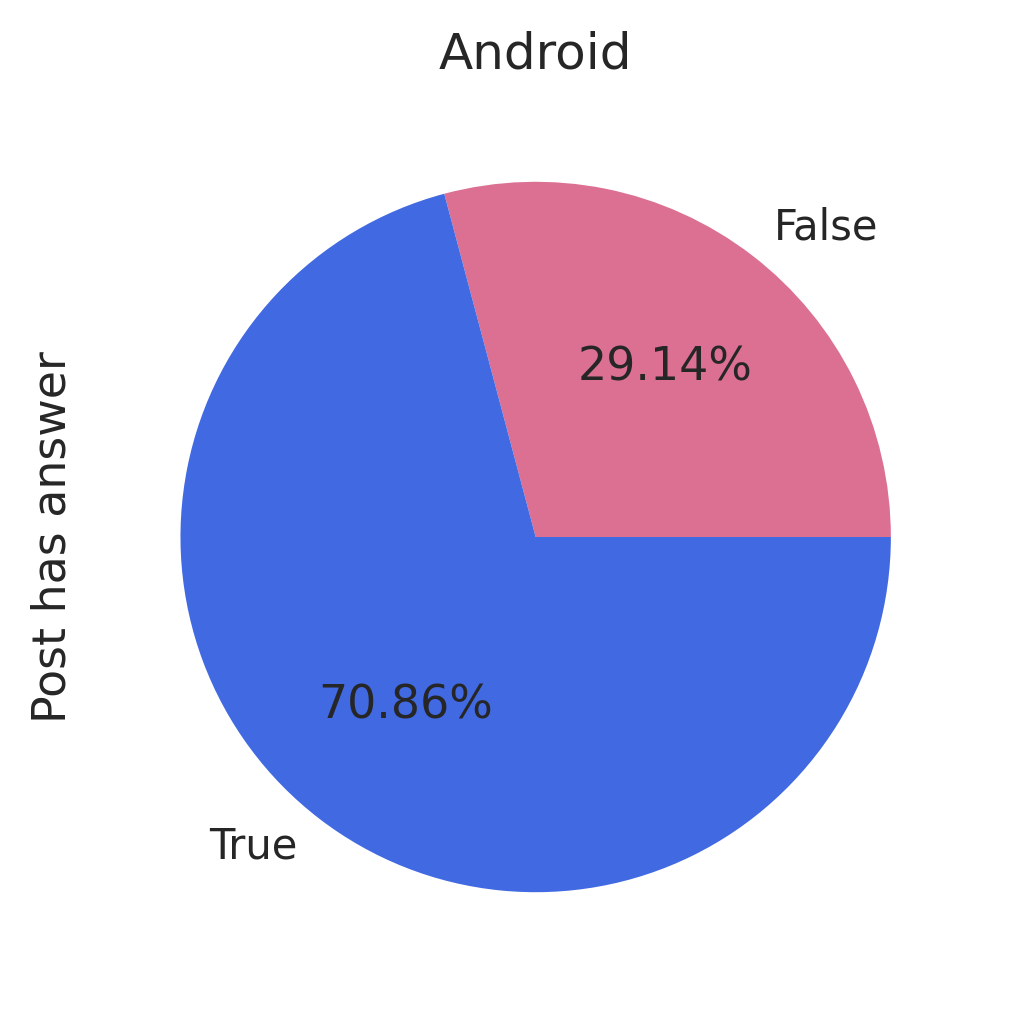
\includegraphics[width=0.45\textwidth]{android-vs-ios/android_answer.png} }}%
    \qquad
    \subfloat{{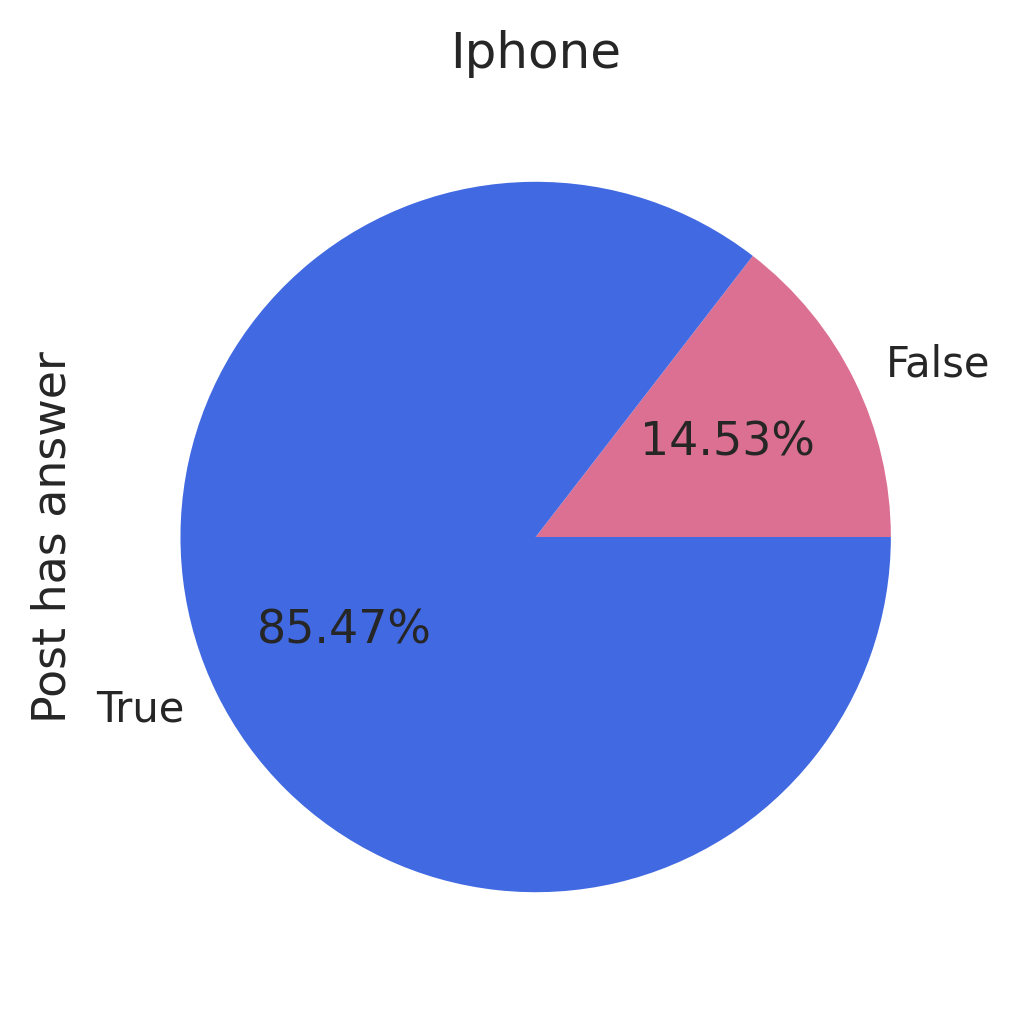
\includegraphics[width=0.45\textwidth]{android-vs-ios/iphone_answer.png} }}%
    \caption*{Porównanie względnej liczby postów, które dostały odpowiedź}
    \label{fig:example}%
\end{figure}
    
\end{frame}

\begin{frame}{Posty, które mają \textit{zaakceptowaną} odpowiedź}

\begin{figure}%
    \centering
    \subfloat{{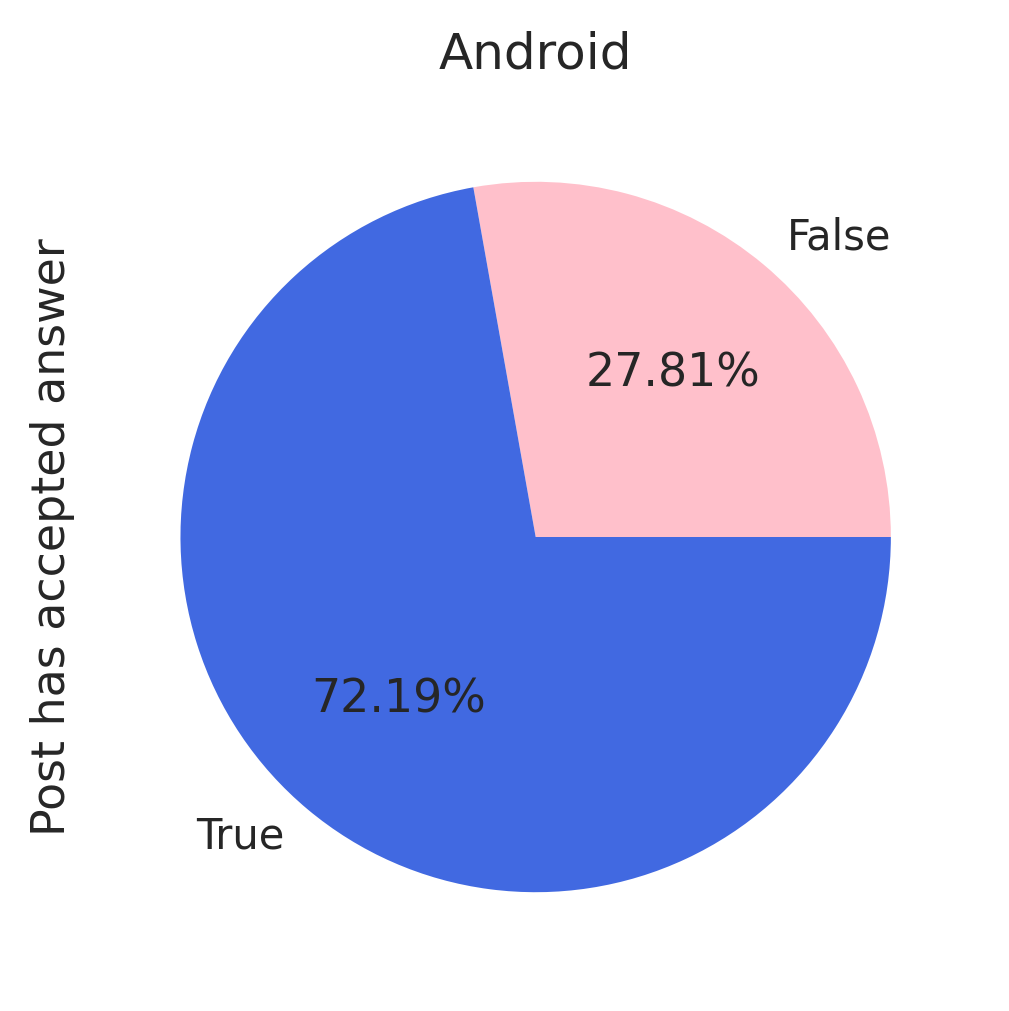
\includegraphics[width=0.45\textwidth]{android-vs-ios/android_accepted.png} }}%
    \qquad
    \subfloat{{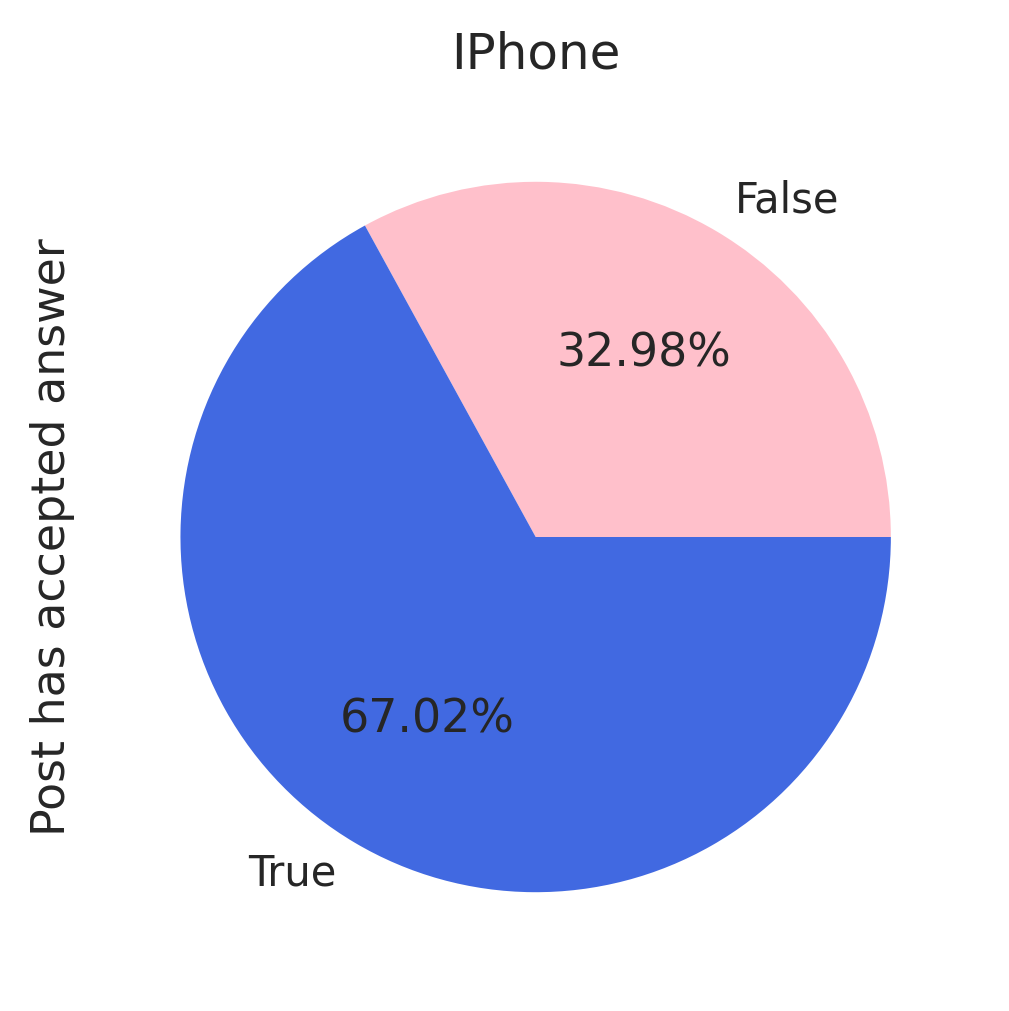
\includegraphics[width=0.45\textwidth]{android-vs-ios/iphone_accepted.png} }}%
    \caption*{Porównanie względnej liczby postów, które dostały \textit{zaakceptowaną} odpowiedź}
    \label{fig:example}%
\end{figure}
    
\end{frame}

\begin{frame}{Android vs iOS - wnioski}
    \begin{itemize}
        \item użytkownicy iOS-a są bardziej pomocną społecznością (więcej postów z udzieloną odpowiedzią)
        \item może to wynikać z tego, że jest więcej użytkowników serwisu Apple'a (ale nie musi)
        \item natomiast posty na forum Androida mają względnie więcej zaakceptowanych odpowiedzi
        \item możliwe, że forum Androida posiada więcej ekspertów i odpowiedzi są trafniejsze
    \end{itemize}
\end{frame}

\end{document}